\pagestyle{empty}
\section{System Testing \\{\small\tt{J.~Pearse}}}
The behaviour of the simulation was verified and tested using a combination of the diagnostic tools integrated into the visualisation and diagnostic functions exported from Erlang modules. Entity behaviours which arising from interactions were observed and investigated. The highly concurrent nature of the simulation presents some particular challenges.

\subsection{Simulation reporting}
The report function of the environment module builds a list of entity data gathered from each tile, the tile keeps details of the entity states so the compiled list contains a snap-shot of all entity states. However some time will elapse between the time the environment calls one tile and another.
\begin{enumerate}
\item{environment calls Tile A and adds its state to the report, entities on Tile B are still moving}
\item{environment calls Tile B and concatenates this with the report from tile A, entities on Tile A meanwhile may have moved}
\end{enumerate}
Matters are further complicated by the independent states of entities, before an entity moves it updates its state by calling the viewer to examine its surroundings, then it calls the tile with its updated position - in the meantime other entities will have called the tile with their updated positions.
Any given report submitted from the environment consists of many entity states, captured at slightly differing times. Although the report has such discrepancies in the data, the simulation itself does not rely on the report data for any function.
\subsection{Visualisation}
Every object drawn in the visualisation uses data from the WebSocket report which is very helpful in understanding the state of the simulation. The SVG format uses a coordinate system with the \( \{ 0,0 \} \) origin in the top-left corner, this same system is used in the simulation internal co-ordinates facilitating the direct mapping of simulation positions to visualisation elements. 
\begin{figure}[h]
  \centering
  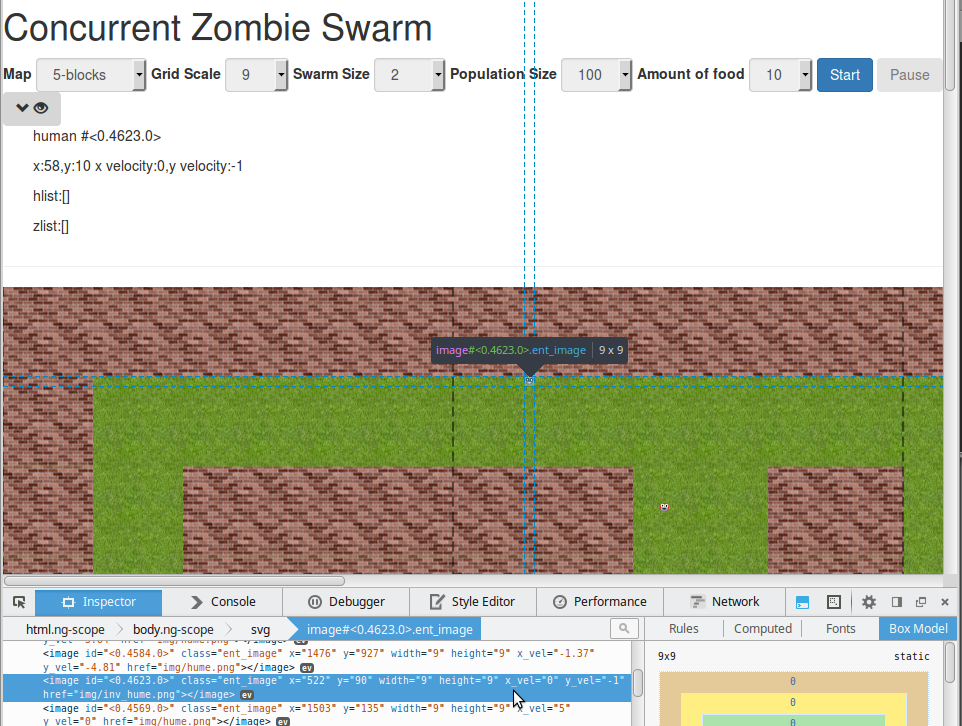
\includegraphics[width=0.9\textwidth]{img/co-ordinates.png}
\caption{Co-ordinate mapping}
    \label{fig:co-ordinate mapping}
\end{figure}
The position values are multiplied with a magnification value for the visualisation, set by the Grid Scale drop-down - here set at \(9\) as we can see arbitary attributes (such as y\_vel) can be assigned to each element of the SVG.
There is animated 'tweening' between reports which sometimes causes the appearance of entities cutting corners in the animation. The speed of individual entities is clearly observable in the visualiser allowing us to see the effect of energy-loss slowing them down gradually and then speeding up again when they gain more energy.
\subsection{Inspection panel}
The inspection panel displays elements from the state of any entities selected in the visualiser. By pausing the simulation and clicking on an entity, the process id of the entity can be determined and used to call any exported functions from the Erlang console.
\subsection{Line of sight}
A graphical representation of each entity selected is drawn into the SVG, the interesting aspect of the LOS visualisation is the way it reveals the concurrency inherent in the system, lines are not always drawn to the exact position where entities are, because lines are drawn based on the selected entities state they are sometimes drawn to the position their target will be at in the next report cycle although this gives the appearance that the visualisation is out of sync, it's a natural effect of trying to visualise a highly concurrent system in discrete snapshots.
\begin{figure}[f]
  \centering
  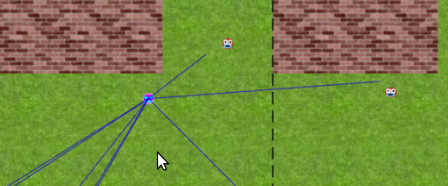
\includegraphics[width=0.7\textwidth]{img/concurrent-lag.png}
\caption{Concurrency visualised}
    \label{fig:Concurrency visualised}
\end{figure}

The enities are drawn from data collected from the tile state but the sight-lines are drawn from positions in the entity state. Which can lead to cross tile lines pointing to the position the entity will be in.
\clearpage
\endinput
